\documentclass[letterpaper,11pt]{article}
\usepackage{graphicx}
\usepackage[margin=0.9in]{geometry}
\usepackage{tabularx}
\usepackage{amsmath}
\usepackage{enumerate}
\usepackage{hyperref}
\usepackage{verbatim}
\usepackage{color}


\renewcommand{\vec}[1]{\mathbf{#1}} % Display vectors as boldface %

\let\oldhat\hat   % Also display hats as boldface
\renewcommand{\hat}[1]{\oldhat{\mathbf{#1}}} % Also display hats as boldface

\begin{document}

\title{Heat transfer from an ultrafast laser heated metal film to a substrate}
\author{Eric Landahl}
%\date{}

\maketitle

\section{Introduction}
This note describes how to calculate one-dimensional thermal transport from an ultrafast laser excited metal film into a substrate.  The laser rapidly  ($\approx$ 1 ps) raises the temperature of the film uniformly.  The film has been depositied on top of a bulk material, which is initially at a uniform colder temperature.   The specific experiments considered are a 70 nm thick Aluminum film sputtered on top of four different bulk semiconducor crystalline wafers:  Silicon, Gallium Arsenide, Indium Antimonide, and Germanium.  The different thermal properties of these bulk semiconductor materials provide a useful comparitive study.  Metal-on-semiconductor devices are important technologically, and we are undertaking a quantituative study of their heat transport using time-resolved x-ray diffraction.  This note describes the different transport models which can be used to simulate the results of the diffraction experiments. 

\section{Classical Treatment}

\subsection{Perfect thermal contact}

These results are taken from Example 10.8 of Hahn and Ozisik, \emph{Heat Conduction} (Wiley, 2012).  They consider a one-dimensional, two-layer composite slab with a film  of thickness $L$ on top of a semi-infinite bulk material.   We will identify the film as region 1 and the bulk as region 2.   The layers are presumed to be in perfect thermal contact with region 1 initially at a uniform temperature $T_0$ (caused by rapid laser energy absorption) and region 2 at zero temperature.  The problem is easiest stated using a dimensionless temperature $\theta_i(x,t)$ defined as as
\begin{equation}
\theta_i(x,t) = \dfrac{T_i(x,t)}{T_0} \hspace{0.5in} i = 1,2 
\end{equation}
where the index $i = 1,2$ refers to the film and bulk, respectively.  With this transformation, the heat transfer problem is written
\begin{subequations}
\begin{align}
\dfrac{\partial^2 \theta_1}{\partial x^2} &= \dfrac{1}{\alpha_1}\dfrac{\partial \theta_1}{\partial t} \hspace{0.5in} in \hspace{0.5in} 0<x<L, \; t>0 \\
\dfrac{\partial^2 \theta_2}{\partial x^2} &= \dfrac{1}{\alpha_2}\dfrac{\partial \theta_2}{\partial t} \hspace{0.5in} in \hspace{0.5in} x>L,\; t>0
\end{align}
\end{subequations}
subject to the boundary conditions
\begin{subequations}
\begin{align}
& \dfrac{\partial \theta_1}{\partial x} \Big| _{x=0} = 0 \\
& \theta_1(x=L,t) = \theta_2(x=L,t) \\
& k_1 \dfrac{\partial\theta_1}{\partial x} \Big| _{x=L} = k_2  \dfrac{\partial\theta_2}{\partial x} \Big| _{x=L} \\
& \theta_2(x \rightarrow \infty,t) \rightarrow 0
\end{align}
\end{subequations}
and the initial conditions
\begin{subequations}
\begin{align}
& \theta_1(x, t=0) = 1 \hspace{0.5in} in \hspace{0.5in} 0<x<L \\
& \theta_2(x, t=0) = 0 \hspace{0.5in} in \hspace{0.5in} L<x<\infty
\end{align}
\end{subequations}
where $k_i$ are the thermal conductivities and $\alpha_i$ are the thermal diffusivities of region 1 (film) and region 2 (bulk).  
Using Laplace rransforms, the solution for the temperature distribution in the two-layer medium is
\begin{subequations}
\begin{align}
& \dfrac{T_1(x,t)}{T_0}=1-\dfrac{1+\gamma}{2}\sum\limits_{n=0}^\infty \gamma^n \Bigg\{ \textnormal{erfc} \left[ \dfrac{(2n+1)L-x}{2\sqrt{\alpha_1 t}} \right] + \textnormal{erfc} \left[ \dfrac{(2n+1)L-x}{2\sqrt{\alpha_1 t}} \right] \Bigg\}  \\
& \dfrac{T_2(x,t)}{T_0}=\dfrac{1+\gamma}{2}\sum\limits_{n=0}^\infty \gamma^n \Bigg\{ \textnormal{erfc} \left[ \dfrac{(2nL+\mu(x-L)}{2\sqrt{\alpha_1 t}} \right] - \textnormal{erfc} \left[ \dfrac{(2n+2)L+\mu(x-L)}{2\sqrt{\alpha_1 t}} \right] \Bigg\} 
\end{align}
\end{subequations}
where the unitless parameters $\mu$ and $\gamma$ are defined by
\begin{subequations}
\begin{align}
& \mu = \sqrt{\dfrac{\alpha_1}{\alpha_2}} \\
& \beta = \dfrac{k_1}{k_2} \dfrac{1}{\mu} \\
& \gamma = \dfrac{\beta -1}{\beta+1} .
\end{align}
\end{subequations}

\subsection{Examples of the classical heat conduction result}
We consider a 70 nm Aluminum film directly on top of bulk semiconductors.  In addition to calculating the temperature profile evolution in the film and substate, we perform Time-Resolved X-Ray Diffraction (TRXD) calculations to predict the evolution of Bragg reflection lineshapes following laser excitation.  For each material, the absorbed laser fluence is kept constant at 1 mJ/cm$^2$.  TRXD measurements are all done for single crystal (001) cut semiconductors at the [004] reflection at an x-ray energy of 10 keV.  In these preliminary calculations only the lineshapes, and not the absolute intensiteis of the diffraction profiles are considered, and they are blurred by convolving the results of a dynamical diffraction calculation with a 0.2 millidegree FWHM Gaussian resolution function.  The TRXD calculations should be considered still under development and requiring further benchmarking at this time.  The temperature profiles are calcualated on a logarithmic time grid stretching from 1 ps to 1 $\mu$s.  
\newpage
\subsubsection{Aluminum on Silicon}
The 70 nm thick Aluminum film received an initial temperature rise of 58.3 deg C. After 1 $\mu$s, the average film temperature rise was only 0.4 deg C.  The maximum bulk Silicon temperature rise wass 34.0 deg C.
\begin{figure}
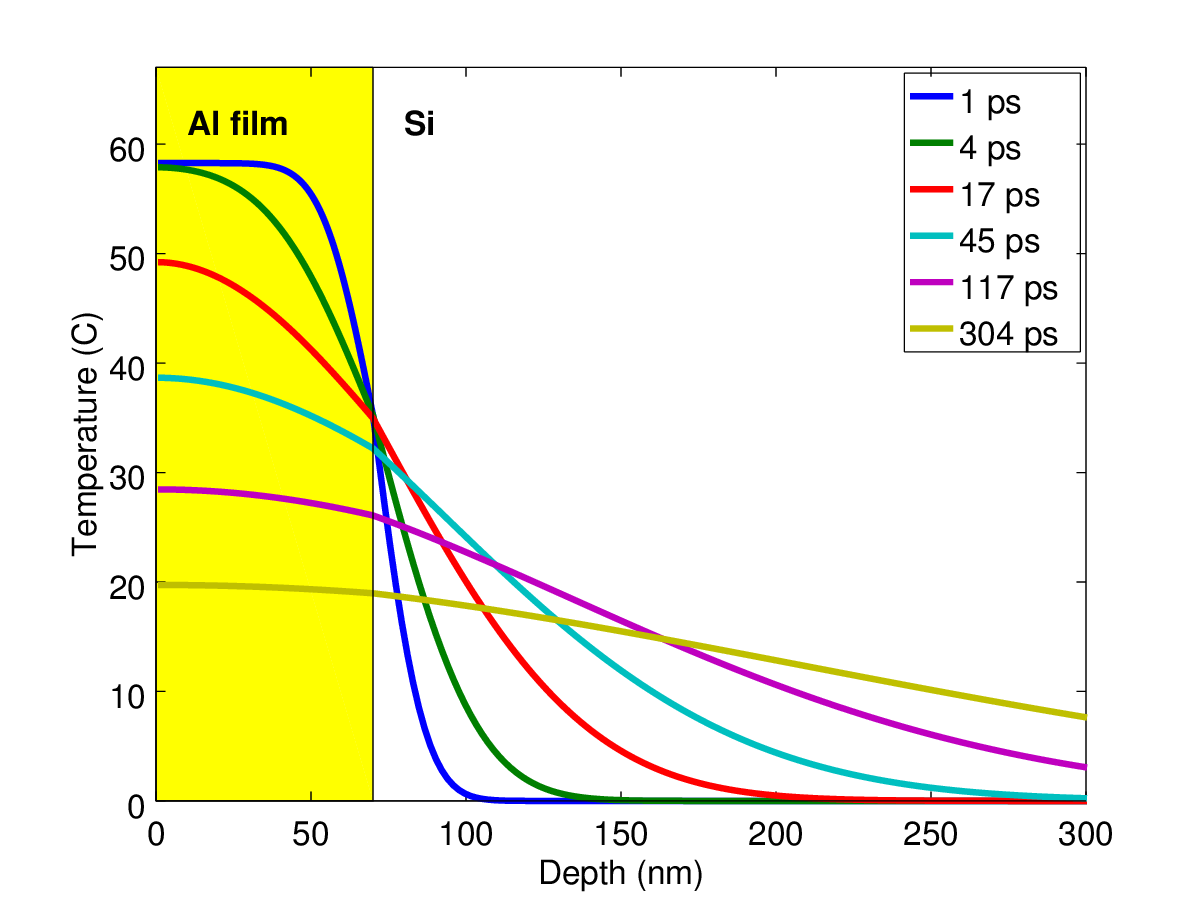
\includegraphics[scale = 0.65]{Si_Temp.png}
\caption{Classical thermal transport result for 70 nm Al on Si.}
\end{figure}
\begin{figure}
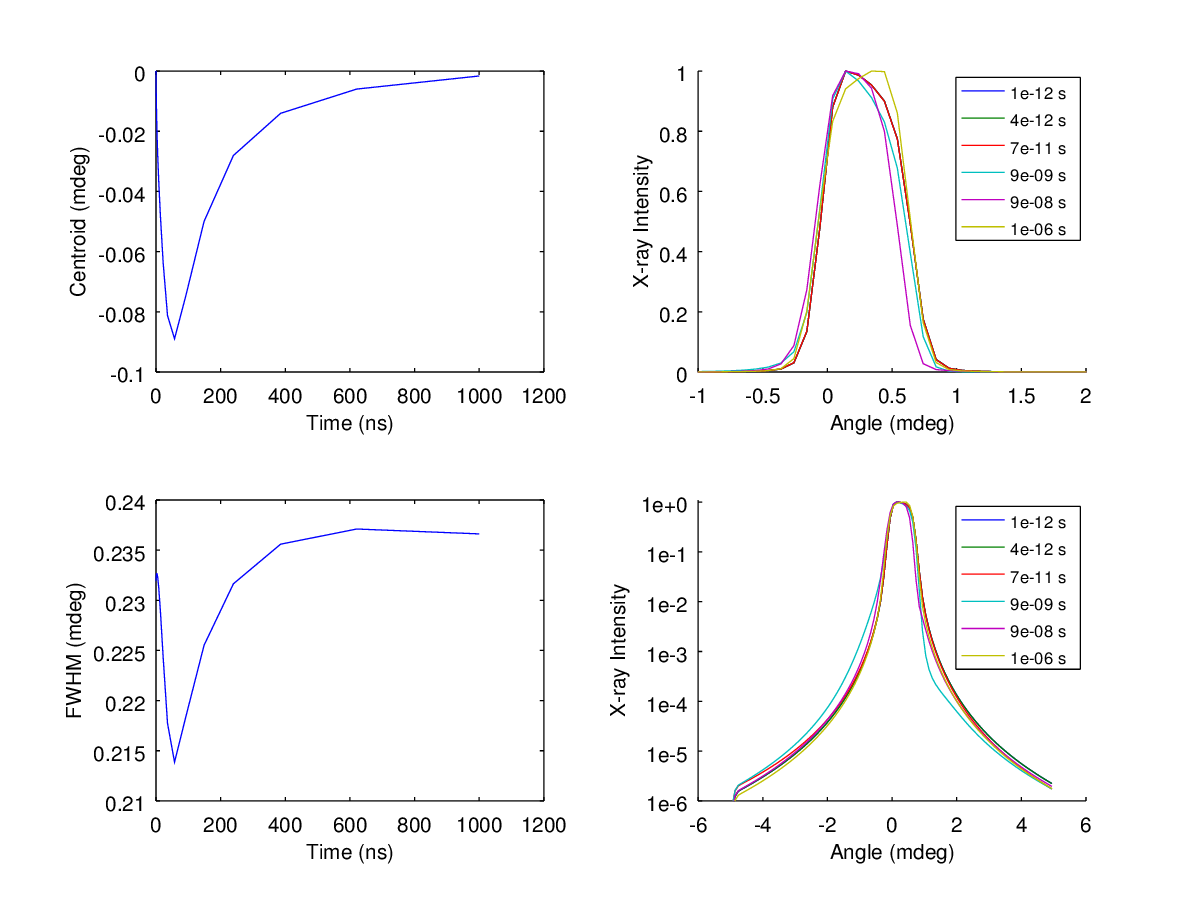
\includegraphics[scale = 0.65]{Si_TRXD.png}
\caption{Preliminary TRXD calculations corresponding to classical thermal transport result for 70 nm Al on Si.}
\end{figure}
\newpage
\subsubsection{Aluminum on Gallium Arsenide}
The 70 nm thick Aluminum film received an initial temperature rise of 58.3 deg C. After 1 $\mu$s, the average film temperature rise was only 0.6 deg C.  The maximum bulk Silicon temperature rise was 39.3 deg C.
\begin{figure}
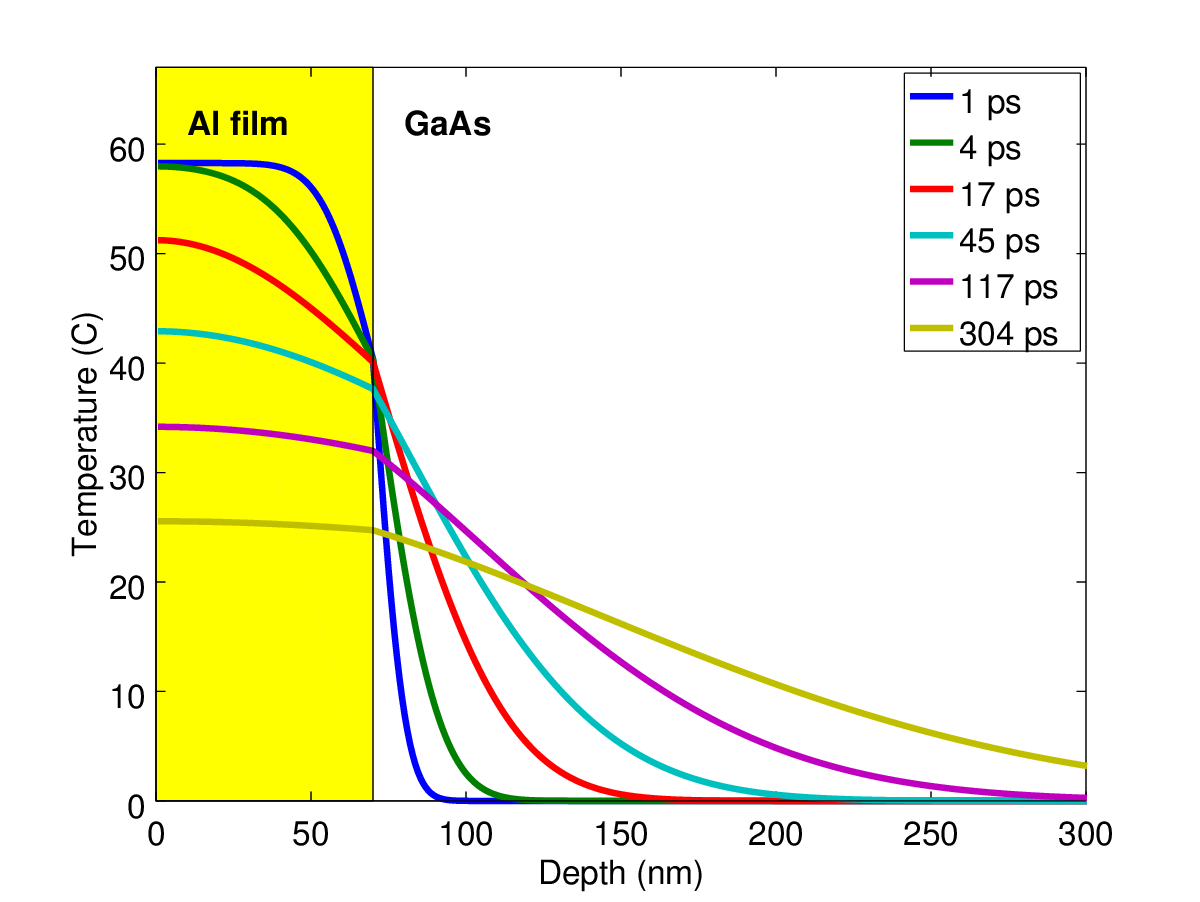
\includegraphics[scale = 0.65]{GaAs_Temp.png}
\caption{Classical thermal transport result for 70 nm Al on Si.}
\end{figure}
\begin{figure}
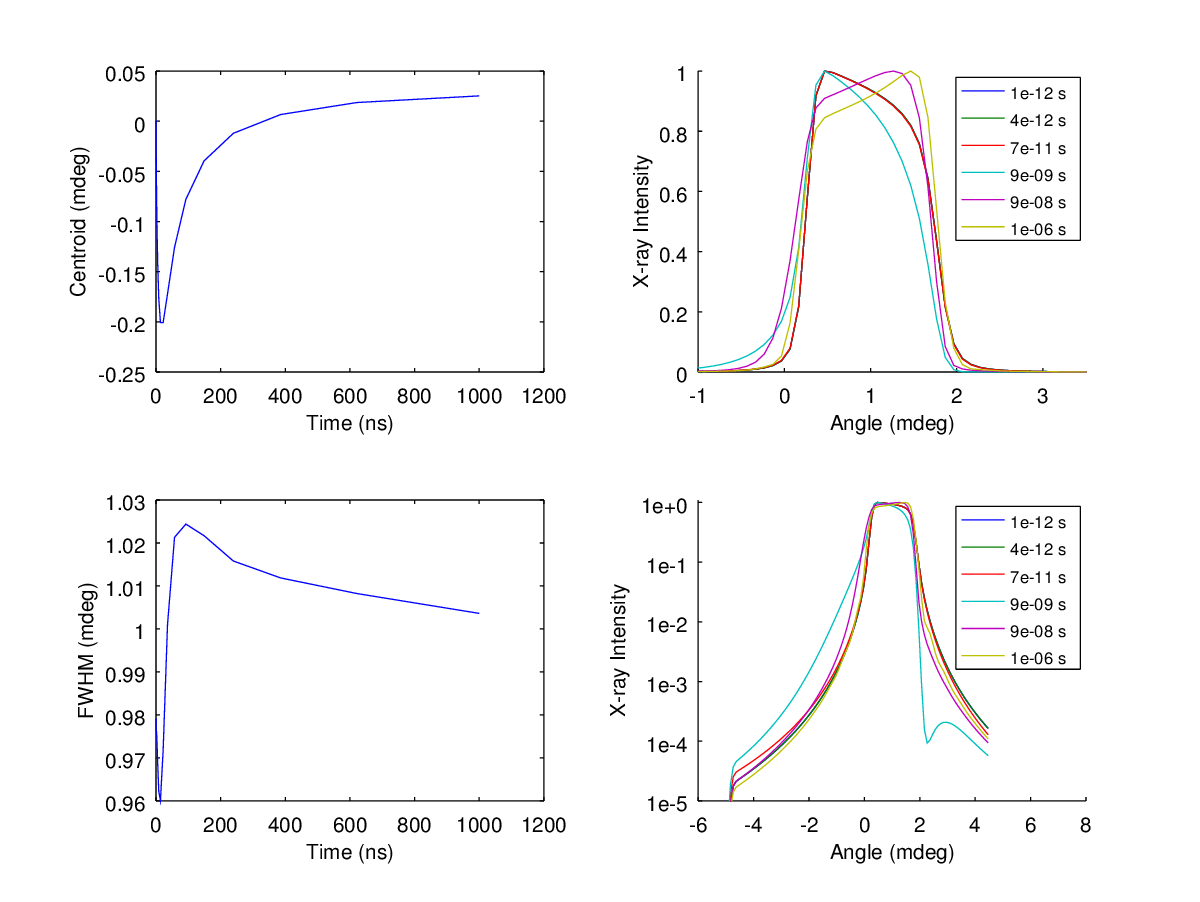
\includegraphics[scale = 0.65]{GaAs_TRXD.png}
\caption{Preliminary TRXD calculations corresponding to classical thermal transport result for 70 nm Al on GaAs.}
\end{figure}
\newpage
\subsubsection{Aluminum on Germanium}
The 70 nm thick Aluminum film received an initial temperature rise of 58.3 deg C. After 1 $\mu$s, the average film temperature rise was only 0.6 deg C.  The maximum bulk Germanium temperature rise was 39.6 deg C.
\begin{figure}
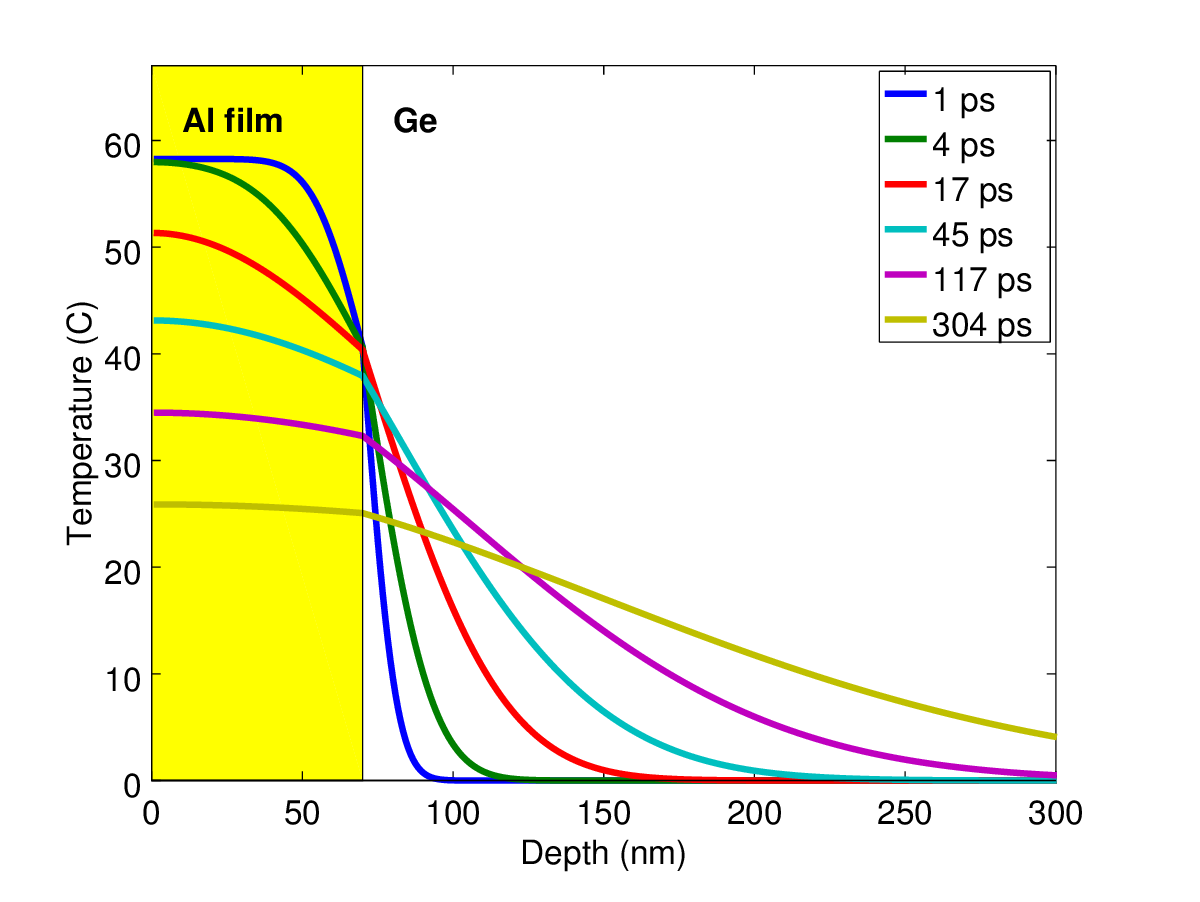
\includegraphics[scale = 0.65]{Ge_Temp.png}
\caption{Classical thermal transport result for 70 nm Al on Si.}
\end{figure}
\begin{figure}
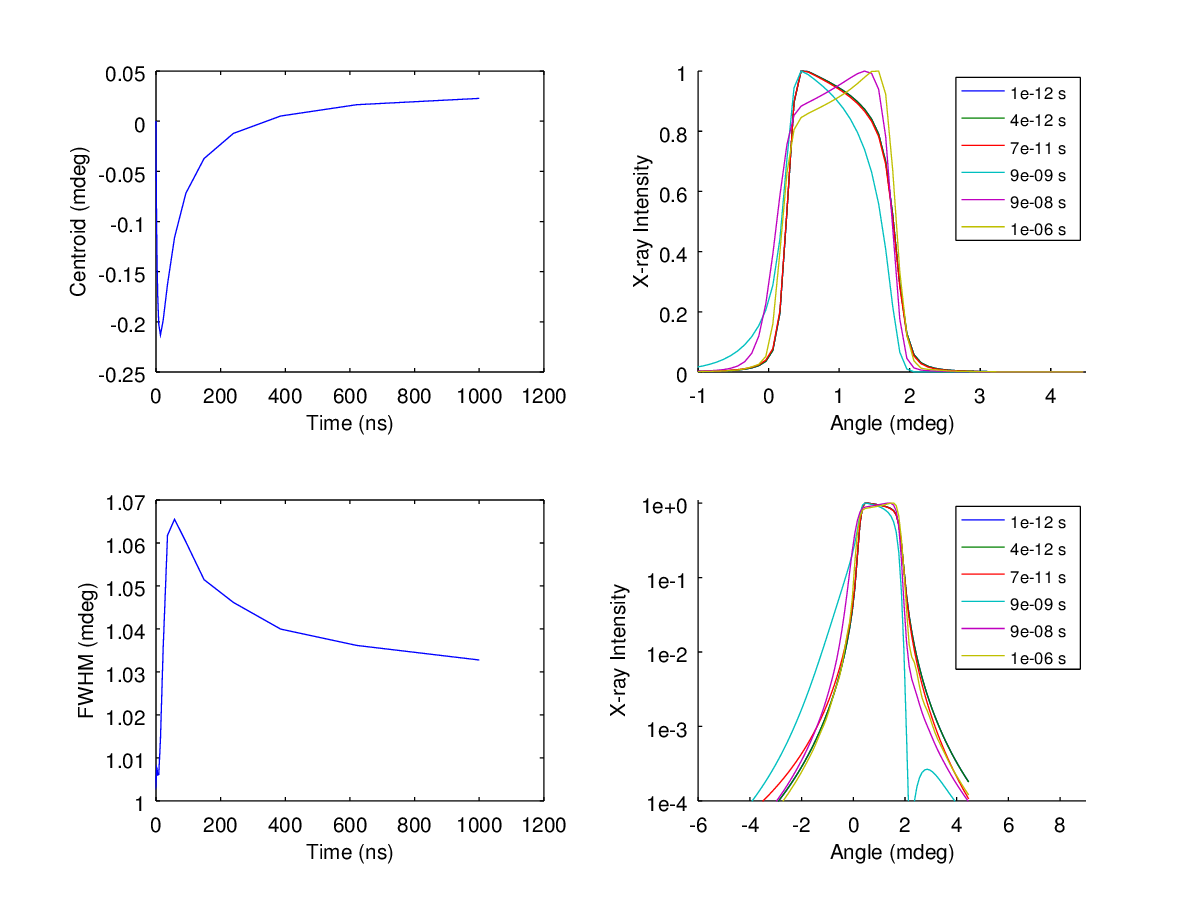
\includegraphics[scale = 0.65]{Ge_TRXD.png}
\caption{Preliminary TRXD calculations corresponding to classical thermal transport result for 70 nm Al on Ge.}
\end{figure}
\newpage
\subsubsection{Aluminum on Indium Antimonide}
The 70 nm thick Aluminum film received an initial temperature rise of 58.3 deg C. After 1 $\mu$s, the average film temperature rise was only 1.2 deg C.  The maximum bulk Indium Antimonide temperature rise was 47.3 deg C.
\begin{figure}
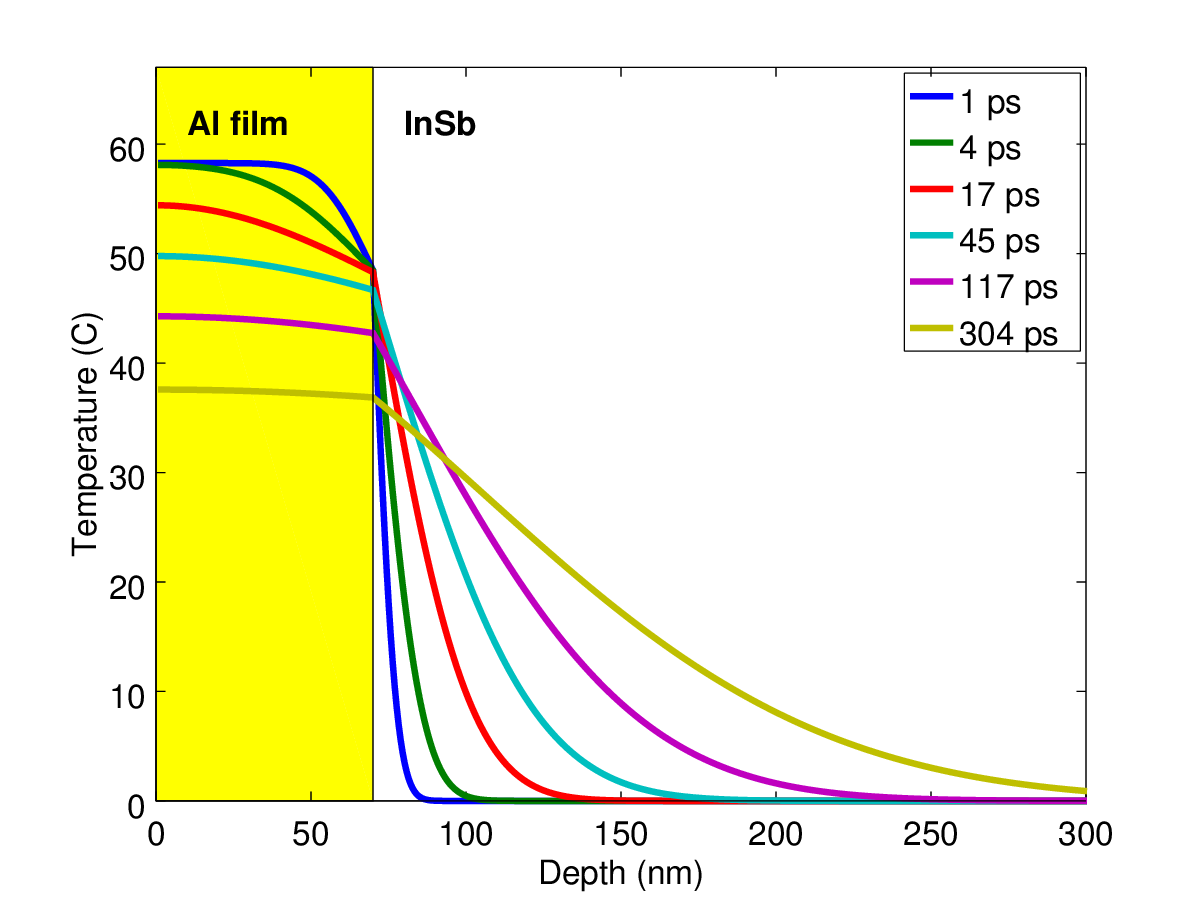
\includegraphics[scale = 0.65]{InSb_Temp.png}
\caption{Classical thermal transport result for 70 nm Al on Si.}
\end{figure}
\begin{figure}
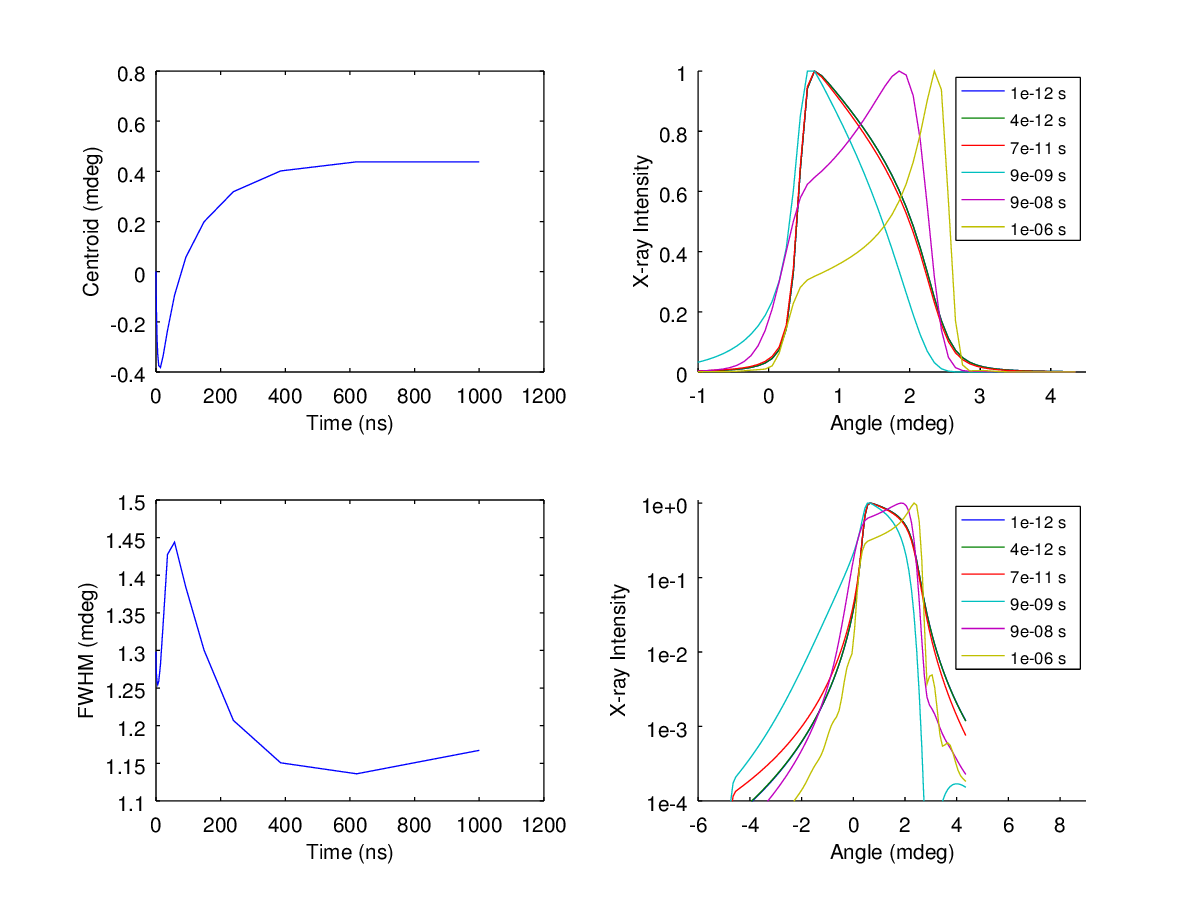
\includegraphics[scale = 0.65]{InSb_TRXD.png}
\caption{Preliminary TRXD calculations corresponding to classical thermal transport result for 70 nm Al on InSb.}
\end{figure}
\newpage
\subsection{Imperfect thermal contact}
This section will explore corrections to the classical treatment due to imperfect thermal contact between the film and substrate.  In particular, the ``Diffusive Mismatch Model" can be used to correct the classical heat conductivity values by applying a locally quantum model of heat flow.  
\section{Microscopic Treatment}
Considerable recent interest in this problem at the 10 - 100 nm lengthscales has been motivated by the semiconductor fabrication techniques working at these dimensions.  The classical treatment given above, even including corrections for interfaces, is known to be insufficient since the phonon mean free path, $\Lambda$, can be comparable to these dimensions.  This section will explain a simple one-dimensional Lattice Boltzman Model (LBM) to treat heat flow as a phonon transport problem.  
\pagebreak

\section*{Appendix: Parameters}

\section*{Appendix: Code}

The most recent and up to date code should be obtained from \url{https://github.com/elandahl/dynamical-diffraction/tree/TRXD/strain_functions}.  This code listing is for reference only. 
 
\verbatiminput{../thermalFilm.m}

\end{document}
